\expandafter\ifx\csname ifdraft\endcsname\relax
    %!TEX encoding = UTF-8
% +++
% latex = "uplatex"
% +++
\documentclass[uplatex,dvipdfmx,b5j,openany]{jsbook}
\usepackage{graphicx}

\usepackage{siunitx}		%for use si unit
\usepackage{here}			%for use figure here
\usepackage{tikz}			%for use TikZ package
\usepackage{pgfplots}		%for use PGFplots
\usepackage{dcolumn}		%for use significant figures in the table
\usepackage{csvsimple}		%for import csv files
\usepackage[RPvoltages,americanresistors,americaninductors,europeanvoltage,americancurrents]{circuitikz}
\usepackage[noto]{pxchfon}	%for use Noto fonts

% To out put TikZ logo
\usepackage{bxtexlogo}
\bxtexlogoimport{TikZ}

\usepackage{wrapfig}
\usepackage[top=1.5cm, bottom=1.5cm, left=2.5cm, right=2cm]{geometry}

% framed settings
\usepackage{framed}
\definecolor{shadecolor}{gray}{0.80}

% mdframed settings
\usepackage[xcolor,framemethod=tikz]{mdframed}
\usetikzlibrary{shadows}
\mdfdefinestyle{bash}{linecolor=black,linewidth=0.5pt}
\mdfdefinestyle{shadow}{linewidth=0pt,backgroundcolor=black!15}

\usepackage[customcolors]{hf-tikz}
\hfsetfillcolor{black!5}
\hfsetbordercolor{black!50}

\usepackage[cache=false]{minted}

\usepackage{uri}

\tikzset{% tikz style set
  	pointtype triangle/.style={mark=triangle*,mark size=4pt},
  	every mark/.style={fill=white,solid},
  	south west label/.style={
		matrix,matrix of nodes,
		anchor=south west,at={(rel axis cs:0.01,0.01)},
		nodes={anchor=west,inner sep=0},
  	},
}

\pgfplotsset{% graph style set
    table/col sep=comma, % Use CSV files
  	compat=1.12,
  	major tick length=0.2cm,
  	minor tick length=0.1cm,
  	every axis/.style={semithick},
  	tick style={semithick,black},
  	legend cell align=left,
  	legend image code/.code={%
		\draw[mark repeat=2,mark phase=2,#1]
	  	plot coordinates {(0cm,0cm) (0.5cm,0cm) (1.0cm,0cm)};
  	},
  	log number format basis/.code 2 args={
	\pgfmathsetmacro\e{#2}
	\pgfmathparse{#2==0}\ifnum\pgfmathresult>0{1}\else
	\pgfmathparse{#2==1}\ifnum\pgfmathresult>0{10}\else
	{$#1^{\pgfmathprintnumber{\e}}$}\fi\fi},
}

% macros
\newcommand{\logoLaTeX}{{\rm \textbf \LaTeX}\hspace{0zw}}
	\graphicspath{{./figure/}}
	\begin{document}
\fi

\chapter{\logoLaTeX 使用環境の構築}
	\logoCiTikZ は\LaTeX の拡張機能ですので、\LaTeX の使用環境を整える必要があります。
	本書の目的は\logoCiTikZ を使用することでありますので、
	本格的な環境構築は行わず、OverleafというWeb上で\LaTeX を使用することができるサービスを使用します。

	\section{Overleafの設定}
		まず、Overleafをブラウザで開きます。URLは以下の通りです。
		\begin{mdframed}[style=shadow]
			\url{https://www.overleaf.com}
		\end{mdframed}\vspace{-3mm}
		すると以下のようなページが開きます。
		\begin{figure}[H]
			\centering
			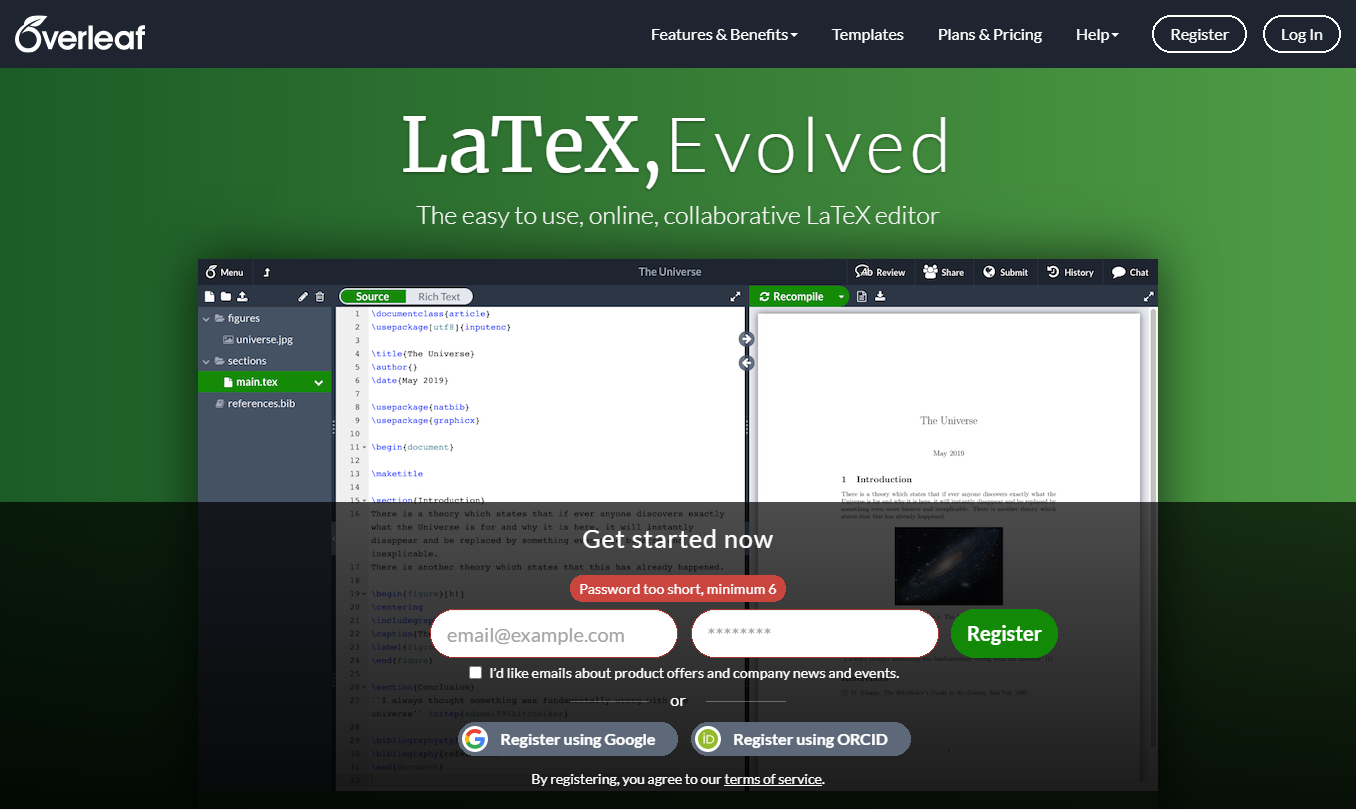
\includegraphics[width=\textwidth]{overleaf-page-top.png}
		\end{figure}
		右上のRegisterをクリックし、会員登録を行います。

		\newpage
		\noindent
		\begin{minipage}{0.4\hsize}%\parindent=1zw
			会員登録が完了すると右のようなページが開くので、
			"Cleate First Project"をクリックし、"Blank Project"を選択します。
			右の図のようなポップアップが出てくるので、ここにProject名を入力します。
			どんな名前でも動作しますが、今回は解説のために
			\begin{mdframed}[style=shadow]
				\url{circuitikz-template}
			\end{mdframed}\vspace{-3mm}
			と入力して、Createをクリックしてください。
		\end{minipage}\hfill
		\begin{minipage}{0.6\hsize}
			\begin{flushright}
				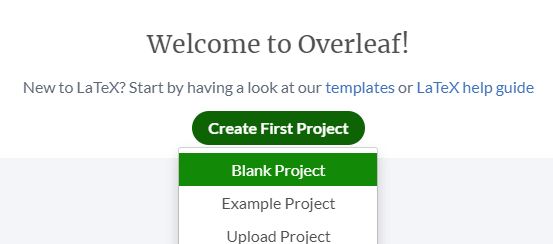
\includegraphics[width=0.95\textwidth]{overleaf-page-createproject.png}\\
				\vspace{3mm}
				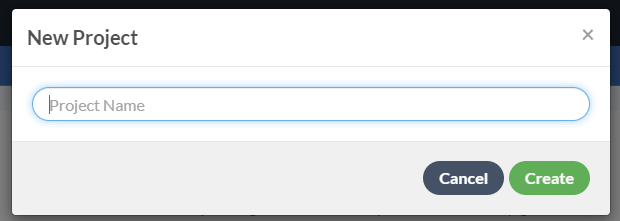
\includegraphics[width=0.95\textwidth]{overleaf-page-projectname.png}
			\end{flushright}
		\end{minipage}
		
		\begin{figure}[H]
			\centering
			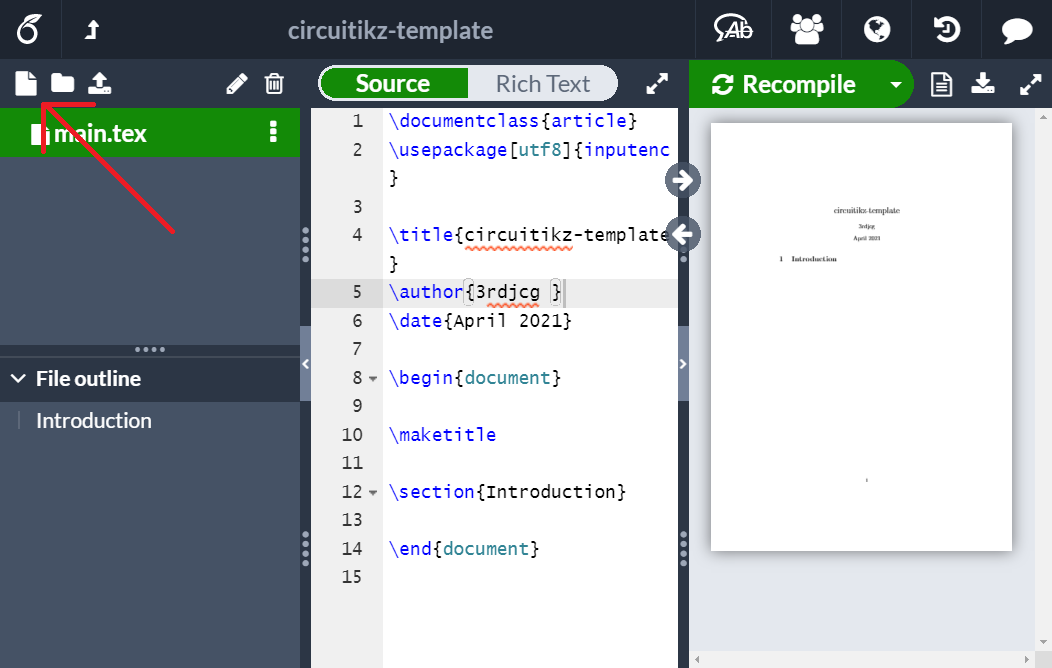
\includegraphics[width=\textwidth]{overleaf-editer-initial.png}
		\end{figure}
		
		\noindent
		\begin{minipage}{0.4\hsize}%\parindent=1zw
			すると上のような画面に遷移しますので、
			赤矢印が示すボタン"New File"をクリックしてください。
			すると右図のような画面が開くので、
			New Fileが選択されていることを確認したうえで
			\begin{mdframed}[style=shadow]
				\url{.latexmkrc}
			\end{mdframed}\vspace{-3mm}
			と入力して、Createをクリックしてください。
		\end{minipage}\hfill
		\begin{minipage}{0.6\hsize}
			\begin{flushright}
				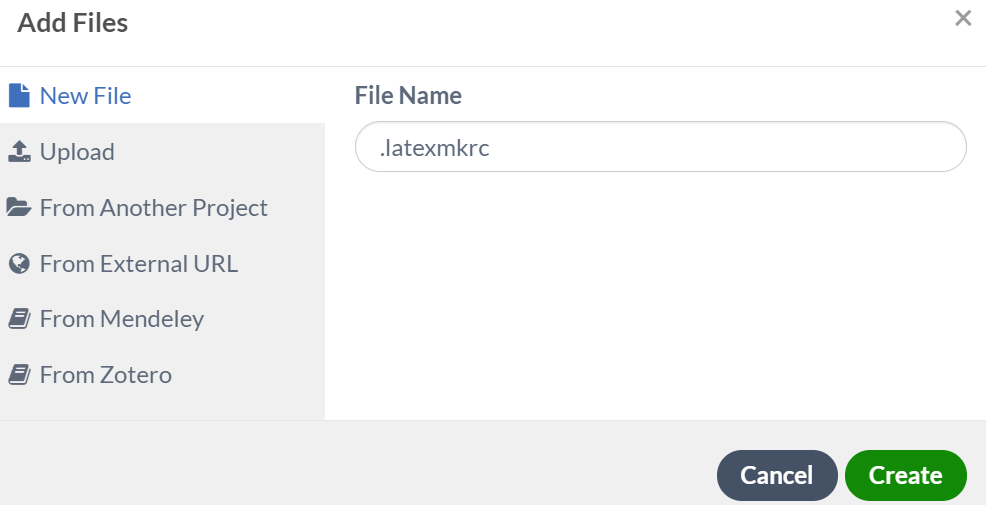
\includegraphics[width=0.95\textwidth]{overleaf-editer-newfile.png}		
			\end{flushright}
		\end{minipage}

		

% 		\newpage
% 		\begin{minted}{perl}
% #!/usr/bin/env perl
% $pdf_mode         = 3;
% $latex            = 'uplatex -kanji=utf8 -no-guess-input-enc -halt-on-error -interaction=nonstopmode -file-line-error --shell-escape';
% $latex_silent     = 'uplatex -kanji=utf8 -no-guess-input-enc -halt-on-error -interaction=batchmode --shell-escape';
% $bibtex           = 'upbibtex';
% $dvipdf           = 'dvipdfmx %O -o %D %S';
% $makeindex        = 'mendex %O -o %D %S';
% 		\end{minted}

\expandafter\ifx\csname ifdraft\endcsname\relax
	\end{document}
\fi